\chapter{Especificación sintáctica}

\section{Introducción}
El objetivo de este capítulo es realizar la especificación sintáctica del lenguaje y mostrar un pseudocódigo de su implementación.

Para llevar acabo la especificación sintáctica, trabajaremos sobre algunos aspectos de la gramática de la sección \ref{sec:definicion_gramatica}, realizando modificaciones que permitan implementar un analizador sintáctico descendente predictivo recursivo sin backtracing.

Luego se hará la implementación en lenguaje Java, haciendo uso del Analizador Léxico del capítulo anterior.

\section{Descripción del problema}
Se requiere realizar una modificación sobre la gramática del lenguaje dada en los capítulos anteriores de manera que se obtenga una gramática equivalente que pueda ser utilizada para desarrollar un analizador sintáctico descendente predictivo recursivo. Para ello, la gramática resultante debe estar factorizada a izquierda, no tener recursividad a izquierda y no debe ser ambigua.

Una vez obtenida la gramática y tratados los posibles conflictos se debe proceder en el diseño de una analizador sintáctico que permite evaluar si una cadena de tokens obtenidos mediante el analizador léxico cumple correctamente con la sintaxis dada en la gramática.

\section{Conflictos de la gramática y el lenguaje}
El análisis sintáctico predictivo recursivo es un método top-down de análisis en el que se ejecutan un conjunto de procedimientos recursivos para procesar la entrada.

Para ello se asocia un procedimiento para cada no terminal de la gramática del lenguaje. Al ser un proceso determinístico, se requiere que la gramática a implementar cumpla con ciertas características para evitar conflictos en el desarrollo del analizador:
\begin{itemize}
\item {\bf Gramática factorizada a izquierda:} exige que solo exista un camino para elegir en un no terminal. Ejemplo de una regla de producción no factorizada a izquierda: $<$A$>$ $\rightarrow$ $<$S$>$ $\alpha$ $|$ $<$S$>$ $\beta$.
\item {\bf Gramática sin recursión a izquierda:} hay dos tipos de recursión a izquierda que deben evitarse: 
\begin{itemize}
\item Cuando se da de manera inmediata en la misma regla de producción: 
\begin{center}
$<$A$>$ $\rightarrow$ $<$A$>$ $\alpha$ $|$ $\beta$
\end{center}
\item Cuando se da a partir de varias reglas de producción:
\begin{center}
$<$S$>$ $\rightarrow$ $<$A$>$ $\beta$\\
$<$A$>$ $\rightarrow$ $<$S$>$ $\alpha$ $|$ $\alpha$
\end{center}
\end{itemize}
\item {\bf Gramática no ambigua:} que exista un único árbol de derivación para una entrada.
\end{itemize}

Las gramáticas que cumplen con estas características son clasificadas en las clases de gramática LL(1). A continuación trataremos de modificar nuestra gramática para que alcance la clase de gramáticas LL(1) o resuelvan estos conflictos mediante un tratamiento especial.

\subsection{Factorización a izquierda}
Para factorizar a izquierda se utilizó el siguiente algoritmo:

\begin{center}
\fbox{\begin{minipage}{14cm}
Sea la regla sin factorización a izquierda:
\begin{center}
$<$A$>$ $\rightarrow$ $\alpha$ $|$ $\alpha$ $<$B$>$
\end{center}
Se procede a reemplazarla por la siguiente construcción, factorizada izquierda, equivalente:
\begin{center}
$<$A$>$ $\rightarrow$ $\alpha$ $<$A$_1$$>$ \\
$<$A$_1$$>$ $\rightarrow$ $<$B$>$ $|$ $\lambda$
\end{center}
Donde $<$A$_1$$>$ es un nuevo no terminal que se genera.
\end{minipage}}
\end{center}

Las reglas a las que se les aplicó la factorización a izquierda se presentan en la lista \ref{list:fac_izq} (para simplificar la lista solo pondremos los no terminales del lado izquierdo de la regla):
\begin{mylist}[H]
\caption{Reglas a las que se le aplica factorización a izquierda.}
\begin{multicols}{3}
\begin{itemize}
\item $<$declaration-block$>$
\item $<$variable-declaration-list$>$
\item $<$procedure-and-function-declaration-list$>$
\item $<$procedure-heading$>$ 
\item $<$function-heading$>$
\item $<$parameter-declaration-list$>$
\item $<$statement-list$>$
\item $<$call-write-read-procedure$>$
\item $<$conditional-statement$>$
\item $<$expression-list$>$
\item $<$identifier-list$>$
\end{itemize}
\end{multicols}
\label{list:fac_izq}
\end{mylist}

A modo de ejemplo mostraremos cómo aplicar este método a la regla  $<$statement-list$>$.

\begin{center}
\fbox{\begin{minipage}{14cm}
Sea la regla no factorizada a izquierda: 
\begin{center}
$<$statement-list$>$ $\rightarrow$ $<$statement$>$ $|$ $<$statement$>$ {\bf ;} $<$statement-list$>$
\end{center}
El resultado tras factorizarla a izquierda es:
\begin{center}
$<$statement-list$>$ $\rightarrow$ $<$statement$>$ $<$statement-list$_1$$>$ \\
$<$statement-list$_1>$ $\rightarrow$ {\bf ;} $<$statement-list$>$ $|$ $\lambda$.
\end{center}
Donde $<$statement-list$_1$$>$ es el nuevo no terminal que se genera con la aplicación del método.
\end{minipage}}
\end{center}

Esto fue aplicado a todas las reglas descritas en la lista \ref{list:fac_izq}.

\subsection{Quitando recursión a izquierda}
Para eliminar la recursión a izquierda se utilizó el siguiente método:

\begin{center}
\fbox{\begin{minipage}{14cm}
Sea la regla con recursión a izquierda inmediata:
\begin{center}
$<$A$>$ $\rightarrow$ $<$A$>$ $\alpha$ $|$ $\beta$
\end{center}
Se procede a reemplazarla por la siguiente construcción, sin recursión a izquierda, equivalente:
\begin{center}
$<$A$>$ $\rightarrow$ $\beta$ $<$A$_1$$>$ \\
$<$A$_1$$>$ $\rightarrow$ $\alpha$ $<$A$_1$$>$ $|$ $\lambda$ 
\end{center}
Donde $<$A$_1$$>$ es un nuevo no terminal.
\end{minipage}}
\end{center}

Las reglas que fueron modificadas para eliminar la recursión a izquierda se presentan en la lista \ref{list:rec_izq} (para simplificar la lista solo pondremos los no terminales del lado izquierdo de la regla):

\begin{mylist}[H]
\caption{Reglas a las que se le elimina la recursión a izquierda.}
\begin{multicols}{3}
\begin{itemize}
\item $<$expression$>$.
\item $<$expression$_1$$>$.
\item $<$expression$_2$$>$.
\item $<$expression$_3$$>$.
\item $<$expression$_4$$>$.
\item $<$expression$_5$$>$.
\end{itemize}
\end{multicols}
\label{list:rec_izq}
\end{mylist}

A modo de ejemplo mostraremos cómo aplicar este método a la regla principal desde la cual comienzan a generarse las expresiones. Como se generan muchos no terminales adicionales, primero cambiamos los nombres para que sean más significativos:
\begin{itemize}
\item $<$expression$>$ fue cambiado por $<$expression-or$>$
\item $<$expression$_1$$>$ fue cambiado por $<$expression-and$>$
\item $<$expression$_2$$>$ fue cambiado por $<$expression-rel$>$
\item $<$expression$_3$$>$ fue cambiado por $<$expression-add$>$
\item $<$expression$_4$$>$ fue cambiado por $<$expression-mult$>$
\item $<$expression$_5$$>$ fue cambiado por $<$factor$>$
\end{itemize}

Ahora mostraremos cómo es el resultado de aplicar el método:

\begin{center}
\fbox{\begin{minipage}{14cm}
Sea la regla con recursividad a izquierda:
\begin{center}
$<$expression-or$>$ $\rightarrow$  $<$expression-or$>$ ``or'' $<$expression-and$>$ $|$ $<$expression-and$>$
\end{center}
El resultado tras quitar la recursión a izquierda es:
\begin{center}
$<$expression-or$>$ $\rightarrow$ $<$expression-and$>$ $<$expression-or$_1$$>$ \\
$<$expression-or$_1$$>$ $\rightarrow$ ``or'' $<$expression-and$>$ $<$expression-or$_1$$>$ $|$ $\lambda$.
\end{center}
Donde $<$expression-or$_1$$>$ es el nuevo no terminal que se genera con la aplicación del método.
\end{minipage}}
\end{center}

Esto fue aplicado a todas las reglas descritas en la lista \ref{list:rec_izq}

\subsection{Ambigüedad del lenguaje}
\label{sec:ambiguedad_lenguaje}
La ambigüedad surge cuando existe más de una forma de derivar una cadena. En este lenguaje, cuando se generan construcciones que contienen \texttt{if-then-else} anidados, se pueden generar dos árboles diferentes de derivación. En las figuras \ref{fig:arbol_sintatico_if_ambiguo_1} y \ref{fig:arbol_sintatico_if_ambiguo_2} se ven los árboles posibles para la derivación del siguiente fragmento de programa en nuestro lenguaje:
\begin{figure}[H]
\begin{minted}[autogobble,linenos,xleftmargin=0.35\textwidth,xrightmargin=0.35\textwidth]{pascal}
	if (cond_1) then
		if (cond_2) then
			code_then
		else
			code_else
\end{minted}
\caption{Fragmento de código con \texttt{if} anidados.}
\label{fig:if_ambiguo}
\end{figure}

\begin{figure}[H]
\centering
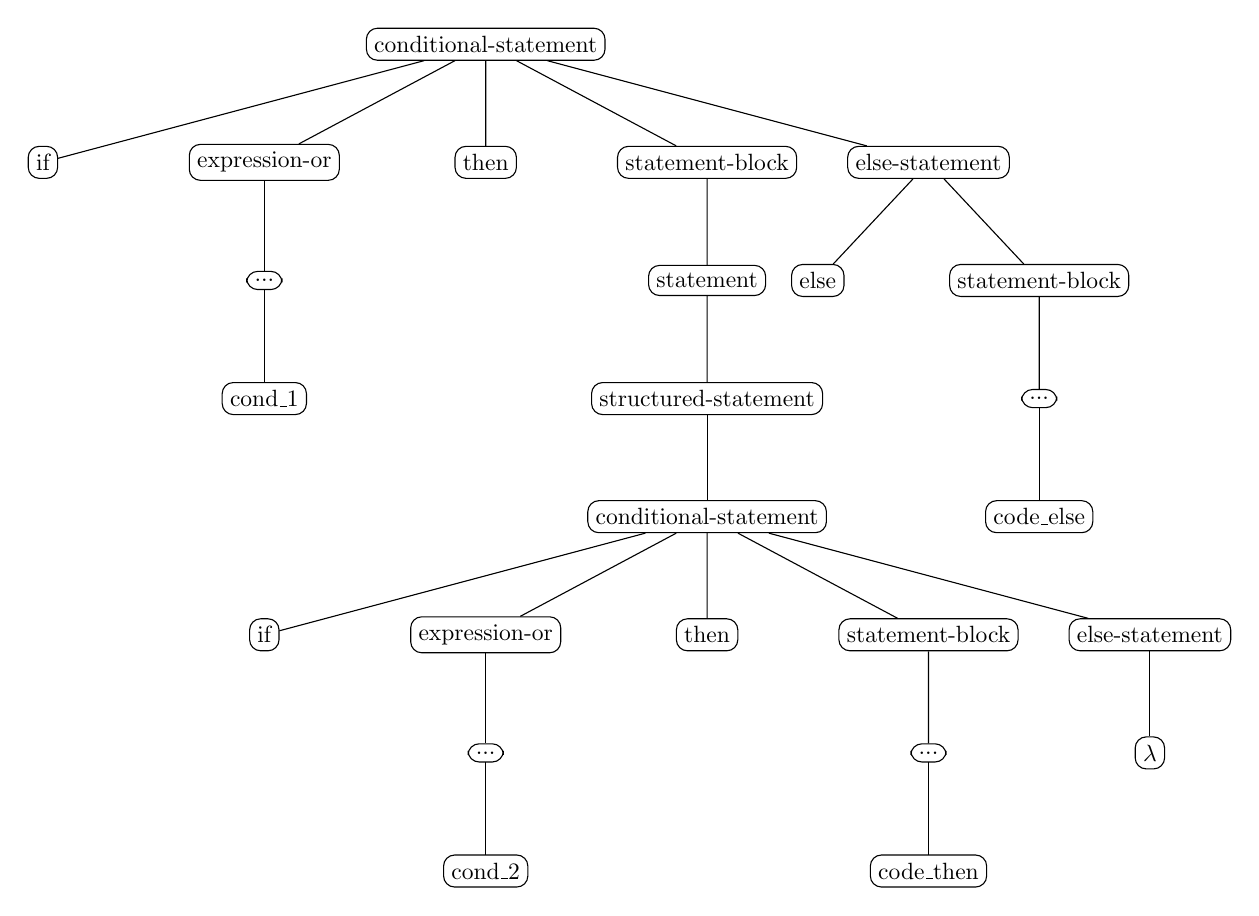
\begin{tikzpicture}[sibling distance=8em,every node/.style = {shape=rectangle, rounded corners,draw, align=center, scale=0.85}]]
\node {conditional-statement}
	child { node {if} }
	child { node {expression-or}
		child { node {...} 
        	child { node {cond\_1} }
        }
	}
	child { node {then} }
    child { node {statement-block} 
    	child { node {statement} 
        	child { node {structured-statement} 
            	child { node {conditional-statement} 
                	child { node {if} }
                    child { node {expression-or}
                    	child { node {...}
                    		child { node {cond\_2} }
                        }
					}
                    child { node {then} }
                    child { node {statement-block}
                    	child { node {...} 
                    		child { node {code\_then} }
                        }
					}
                    child { node {else-statement} 
                    	child { node {$\lambda$} } 
					}
				}
			}
		}
	}
    child { node {else-statement}
    	child { node {else} }
		child { node {statement-block}
        	child { node {...}
        		child { node {code\_else} }
            }
        } 
	};
\end{tikzpicture}
\caption{Árbol de derivación $A$ para la construcción \texttt{if-then-else}.}
\label{fig:arbol_sintatico_if_ambiguo_1}
\end{figure}

\begin{figure}[H]
\centering
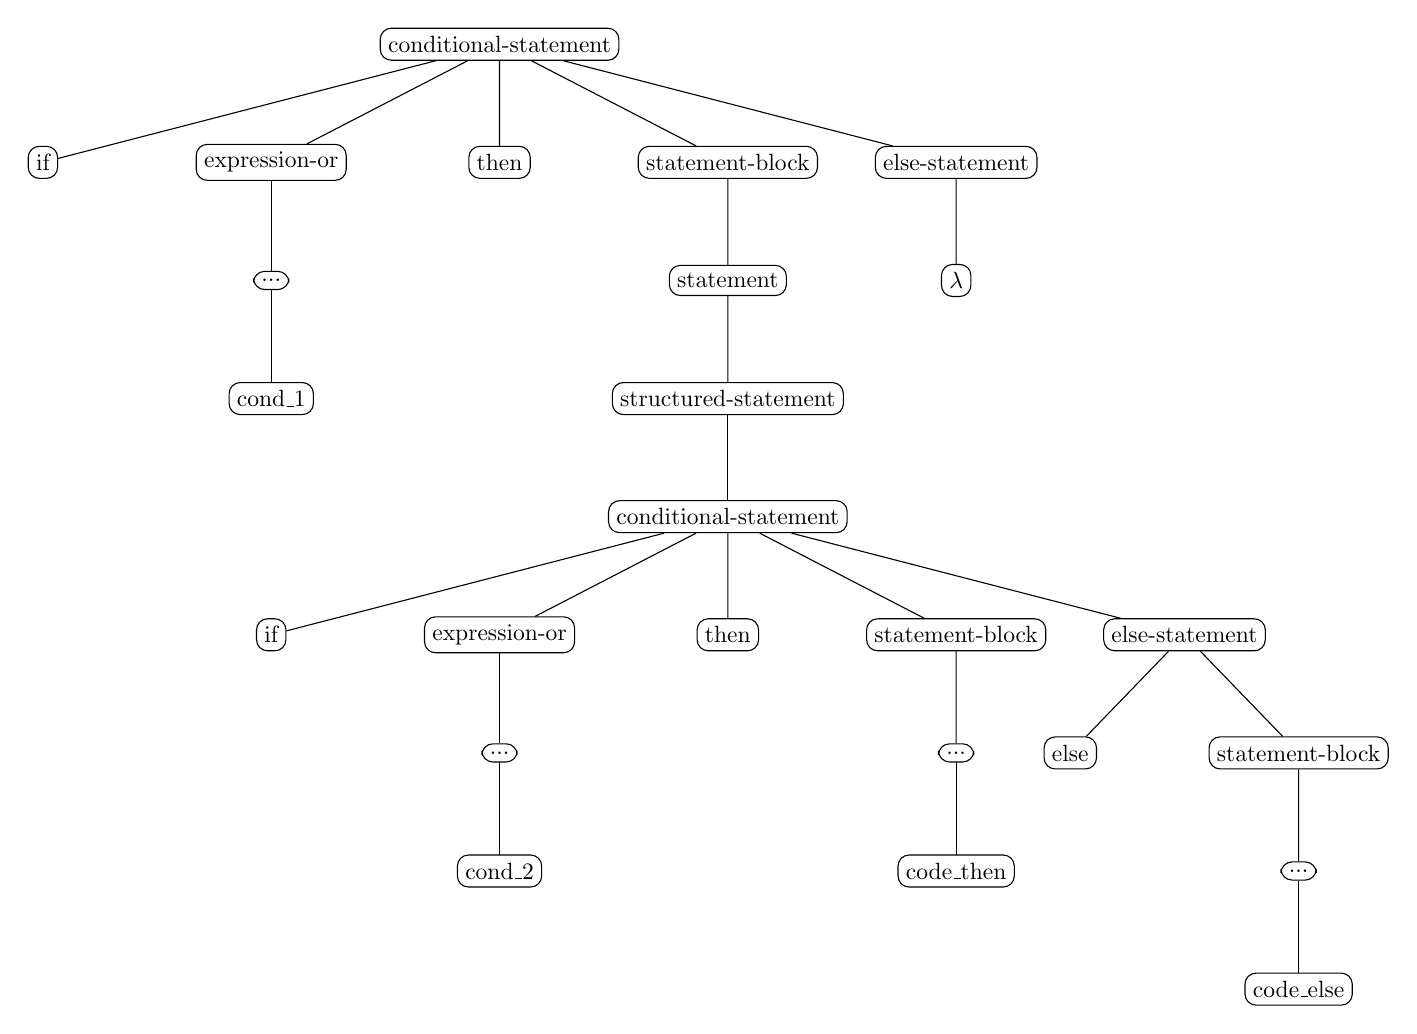
\begin{tikzpicture}[sibling distance=8.25em,every node/.style = {shape=rectangle, rounded corners,draw, align=center, scale=0.85}]]
\node {conditional-statement}
	child { node {if} }
	child { node {expression-or}
    	child { node {...}
			child { node {cond\_1} } 
        }
	}
	child { node {then} }
    child { node {statement-block} 
    	child { node {statement} 
        	child { node {structured-statement} 
            	child { node {conditional-statement} 
                	child { node {if} }
                    child { node {expression-or}
                    	child { node {...}
                    		child { node {cond\_2} }
                        }
					}
                    child { node {then} }
                    child { node {statement-block}
                    	child { node {...}
                    		child { node {code\_then} }
                        }
					}
                    child { node {else-statement}
   					 	child { node {else} }
						child { node {statement-block}
                        	child { node {...}
        						child { node {code\_else} }
                            }
        				} 
					}
				}
			}
		}
	}
    child { node {else-statement}
		child { node {$\lambda$} } 
	};
\end{tikzpicture}
\caption{Árbol de derivación $B$ para la construcción \texttt{if-then-else}.}
\label{fig:arbol_sintatico_if_ambiguo_2}
\end{figure}

El problema surge al momento de decidir si el código correspondiente al \texttt{else} se corresponde con el \texttt{if} interno o el externo.
Este inconveniente no permite que la gramática alcance la clase de gramáticas LL(1). Sin embargo, se puede forzar la implementación del analizador sintáctico para que tome por un camino específico cuando se encuentra esta construcción. La forma más natural es la de la figura \ref{fig:arbol_sintatico_if_ambiguo_2}, donde se asocia el \texttt{else} al \texttt{if} más interno en la estructura de \texttt{if} anidados. Esta es la forma que adoptaremos en la implementación de nuestro analizador.

\section{Gramática modificada}
\label{sec:gramatica_mod}
En esta sección se muestra la gramática con las modificaciones que fueron posibles realizar. 

Se eliminó la recursión a izquierda inmediata y también se factorizó a izquierda. 

Además se eliminó un problema que surgía en el no terminal $<$expression$_{5}$$>$, ya que desde este se podía derivar en $<$identifier$>$ y en $<$call-procedure-or-function$>$, y este último también derivaba en $<$identifier$>$, lo que ocasionaba problemas de factorización a izquierda.

El único inconveniente es que no es posible eliminar la ambigüedad, ya que esta es inherente al lenguaje que está siendo especificado. En la sección \ref{sec:ambiguedad_lenguaje} se mostró dónde surge la ambigüedad.
 
\begin{grammar}
		[(colon){$\rightarrow$}]
		[(semicolon)$|$]
		[(comma){}]
		[(period){\vspace{0.3cm} \\}]
		[(quote){\begin{bf}}{\end{bf}}]
		[(nonterminal){$<$}{$>$}]
		
		%<expression> : <number> ; <number>, [\{"asd"\}], <relational\_operator>, <number>.
		%<number> : <digit> ; <digit> , <number>.
		%<digit> : "0";"1";"2";"3";"4";"5";"6";"7";"8";"9".
		%<relational\_operator> : $"="$;"$\lessthan \greaterthan$";"$\lessthan$";"$\greaterthan$"; "$\lessthan=$";"$\greaterthan=$";"in".
		
		<program> : <program-heading> <block> ".".
		<program-heading> : "program" <identifier> ";".
		<block> : <declaration-block> <multiple-statement> ; <multiple-statement>.
		<declaration-block> : <variable-declaration-block> <declaration-block$_1$> ; <declaration-block$_1$>.
        <declaration-block$_1$> : <procedure-and-function-declaration-list> ; $\lambda$.
		<variable-declaration-block> : "var" <variable-declaration-list>.
		<variable-declaration-list> : <variable-declaration> ";" <variable-declaration-list$_1$>.
        <variable-declaration-list$_1$> : <variable-declaration-list> ; $\lambda$.
		<variable-declaration> : <identifier-list> ":" <type>.
		<procedure-and-function-declaration-list> : <procedure-declaration> ";" <procedure-and-function-declaration-list$_1$> ; <function-declaration> ";" <procedure-and-function-declaration-list$_1$>.
        <procedure-and-function-declaration-list$_1$> : <procedure-and-function-declaration-list> ; $\lambda$.
		<procedure-declaration> : <procedure-heading> ";" <block>.
		<procedure-heading> : "procedure" <identifier> <parameters>.
		<function-declaration> : <function-heading> ";" <block>.
		<function-heading> : "function" <identifier> <parameters> ":" <type>.
        <parameters> : "(" <parameters$_1$> ")" ; $\lambda$.
        <parameters$_1$> : <parameter-declaration-list> ; $\lambda$.
		<parameter-declaration-list> : <parameter-declaration> <parameter-declaration-list$_1$>.
        <parameter-declaration-list$_1$> : "," <parameter-declaration-list> ; $\lambda$.
		<parameter-declaration> : <identifier-list> ":" <type>.
        <statement-block> : <statement> ; <multiple-statament>.
		<multiple-statement> : "begin" <statement-list> "end".
		<statement-list> : <statement> <statement-list$_1$>.
        <statement-list$_1$> : ";" <statement-list> ; $\lambda$.
		<statement> : <simple-statement> ; <structured-statement>.
		<simple-statement> : <identifier> <simple-statement$_1$> ; "write" <call-procedure-or-function> ; "read" <call-procedure-or-function>.
        <simple-statement$_1$> : <assignment-statement> ; <call-procedure-or-function> ; $\lambda$.
		<structured-statement> : <conditional-statement> ; <repetitive-statement>.
		<assignment-statement> : ":=" <expression-or>.
        <call-procedure-or-function> : "(" <call-procedure-or-function$_1$> ")".
        <call-procedure-or-function$_1$> : <expression-list> ; $\lambda$.
		<conditional-statement> : "if" <expression-or> "then" <statament-block> <else-statement>.
        <else-statement> : "else" <statement-block> ; $\lambda$.
		<repetitive-statement> : "while" <expression-or> "do" <statament-block>.
		<expression-list> : <expression-or> <expression-list$_1$>.
        <expression-list$_1$> : "," <expression-list> ; $\lambda$.
        <expression-or> :  <expression-and> <expression-or$_1$>.
        <expression-or$_1$> : "or" <expression-and> <expression-or$_1$> ; $\lambda$.
		<expression-and> : <expression-rel> <expression-and$_1$>.
		<expression-and$_1$> : "and" <expression-rel> <expression-and$_1$> ; $\lambda$.
        <expression-rel> : <expression-add> <expression-rel$_1$>.
        <expression-rel$_1$> : <relational-operator> <expression-add> <expression-rel$_1$> ; $\lambda$.
		<expression-add> : <expression-mult> <expression-add$_1$>.
		<expression-add$_1$> : <addition-operator> <expression-mult> <expression-add$_1$> ; $\lambda$.
        <expression-mult> : <factor> <expression-mult$_1$>.
        <expression-mult$_1$> : <multiplication-operator> <factor> <expression-mult$_1$> ; $\lambda$.
		<factor> : <identifier> <factor$_1$> ; "(" <expression-or> ")" ; <unary-operator> <factor> ; <literal>.
        <factor$_1$> : <call-procedure-or-function> ; $\lambda$.
		<relational-operator> : "$=$" ; "$<>$" ; "$<$" ; "$<=$" ; "$>$" ; "$>=$".
        <unary-operator> : $-$ ; "not".
		<addition-operator> : "$+$" ; "$-$".
		<multiplication-operator> : "$*$" ; "$/$".
		<type> : "integer" ; "boolean".
		<identifier-list> : <identifier> <identifier-list$_1$>.
        <identifier-list$_1$> : "," <identifier-list> ; $\lambda$.
		<identifier> : <letter> <identifier$_1$> ; \_ <identifier$_1$> .
        <identifier$_1$> : <word> <identifier$_1$> ; <number> <identifier$_1$> ; $\lambda$.
		<literal> : <bool> ; <number>.
		<number> :  <digit> <number$_1$>.
		<number$_1$> : <digit> <number$_1$> ; $\lambda$.
        <word> : <letter> <word$_1$> ; "\_" <word$_1$>.
		<word$_1$> : "\_" <word$_1$> ; <letter> <word$_1$> ; $\lambda$.
		<letter> : "A" ; "B" ; "C" ; "D" ; "E" ; "F" ; "G" ; "H" ; "I" ; "J" ; "K" ; "L" ; "M" ; "N" ; "O" ; "P" ; "Q" ; "R" ; "S" ; "T" ; "U" ; "V" ; "W" ; "X" ; "Y" ; "Z" ; "a" ; "b" ; "c" ; "d" ; "e" ; "f" ; "g" ; "h" ; "i" ; "j" ; "k" ; "l" ; "m" ; "n" ; "o" ; "p" ; "q" ; "r" ; "s" ; "t" ; "u" ; "v" ; "w" ; "x" ; "y" ; "z".
		<digit> : "0" ; "1" ; "2" ; "3" ; "4" ; "5" ; "6" ; "7" ; "8" ; "9".
		<bool> : "true" ; "false".
\end{grammar}

\section{Estrategias}
%esto no se si ponerlo aca, en la conclusion, o no ponerlo. ESTA BIEN ACA xd
Al tener que realizar muchos cambios sobre la gramática, era probable cometer errores, por lo que primero decidimos cambiar los nombres de algunos no terminales para que sean mas expresivos, y luego aplicamos la factorización a izquierda y después la eliminación de la recursión a izquierda. Estos dos algoritmos podrían haberse realizado en el orden inverso, pero ejecutados en el orden que propusimos nos aseguramos que luego de eliminar la recursividad no se generaran construcciones que no estén factorizadas a izquierda. 

En cuanto a la ambigüedad del lenguaje, como dijimos en \ref{sec:ambiguedad_lenguaje}, tomamos como criterio hacer corresponder el \texttt{else} con el \texttt{if} más interno. 

\section{Limitaciones}
%mas chamuyo por aca JOYA 
La única limitación encontrada fue la expresividad del lenguaje, que hace que algunas construcciones sean ambiguas. Sin embargo no presenta un gran problema, ya que tomamos decisiones que permiten construir el analizador sintáctico descendente. En la siguiente sección mostraremos cómo esta limitación puede ser mitigada.
%fin del chamuyo

\section{Diseño del analizador sintáctico}
\label{sec:diseno_sintactico}
En el apéndice \ref{apx:pseudocodigo_sintactico} se expone el pseudocódigo del analizador sintáctico descendente predictivo recursivo basado en la grámatica modificada dada en la sección \ref{sec:gramatica_mod}. Este dispone de un método \texttt{match} que permite verificar si un terminal de la gramática coincide con el símbolo de preanálisis obtenido a partir del analizador léxico. Por otro lado dispone de un método para cada no terminal de la gramática, donde se evalúa sus conjuntos de Primeros y se determina con qué terminales debe unificar o a qué otros no terminales debe llamar. En caso de no coincidir tales conjuntos de primeros, se procede a lanzar un \texttt{error}, a excepción de los casos donde la gramática acepta $\lambda$ como opción de la producción.


\section{Implementación del aplicativo}
Para la implementación del analizador sintáctico, utilizaremos el pseudocódigo del apéndice \ref{apx:pseudocodigo_sintactico} y mostraremos su implementación en lenguaje Java. Para ello se explicarán algunos procedimientos de ejemplo, y luego el resto de estos serán análogos.

El Analizador Sintáctico trabaja en conjunto con el Analizador Léxico, recibiendo como entrada los tokens que reconozca y devuelva el Analizador Léxico.

Todo lo desarrollado se puede encontrar en el mismo proyecto de GitHub donde está el Analizador Léxico.

\subsection{Descripción del problema}
Para esta etapa requerimos implementar el analizador sintáctico descendente predictivo recursivo, cuya tarea es verificar si la sintaxis de un código fuente cumple las construcciones gramaticales que propone nuestra gramática modificada de la sección \ref{sec:gramatica_mod} y que se corresponda con el pseudocódigo dado en la sección \ref{sec:diseno_sintactico}. 

En caso de que haya un token que no pertenezca a alguna construcción válida, lanzaremos un error adecuado.

Luego de concluir la implementación, mostraremos ejemplos de ejecuciones exitosas y fallidas, como así también las instrucciones para poder utilizar el Analizador Sintáctico.

\subsection{Herramientas utilizadas}
Para desarrollar el programa continuamos desde el mismo proyecto que el Analizador Léxico, en lenguaje Java. La versión de Java sobre la que trabajamos es la 8\footnote{Actualización 171, al día 14/05/2018}(ocho), sobre el sistema operativo Windows 10. 

Continuamos con el proyecto de NetBeans que se encuentra en GitHub.

\subsection{Diseño}
La idea del Analizador Sintáctico es crear un procedimiento para cada no terminal de la gramática, que se encargue de verificar si la sucesión de caracteres de la entrada cumple con la especificación del lenguaje. Al utilizar el analizador léxico, evitaremos recorrer caracter por caracter, y nos centraremos en los tokens recibidos del Analizador Léxico. 

En este sentido expandiremos el proyecto que disponiamos anteriormente, agregando una nueva clase {\bf AnalizadorSintactico}, como se ve en la figura \ref{fig:arbol_dir_3} que dispondrá de los métodos necesarios para llevar a cabo el análisis sintáctico.

\begin{figure}[H]
%no borrar el % de dirtree porque es necesario.
\dirtree{%
.1 src.
.2 compiladorpascal.
.3 CompiladorPascal.java.
.3 lexico.
.3 sintactico.
.4 AnalizadorSintactico.java.
.3 semantico.
}
\caption{Árbol de directorios del proyecto de Java con los archivos del analizador sintáctico.}
\label{fig:arbol_dir_3}
\end{figure}

En el código del AnalizadorSintactico el procedimiento más importante es el \texttt{match}, que verifica si un token recibido de la entrada (el String \texttt{preanalisis}), es igual al token que espera el analizador sintáctico (String \texttt{terminal}). Si son iguales puede continuar avanzando sobre la entrada, y si no son iguales hay un error sintáctico. En la figura \ref{fig:metodo_match} puede verse el código del método \texttt{match}.

\begin{figure}[H]
\begin{minted}[autogobble,linenos,xleftmargin=0.2\textwidth,xrightmargin=0.2\textwidth]{java}
private void match(String terminal) {
	if (preanalisis.getNombre().equals(terminal)) {
		preanalisis = lexico.tokenSiguiente();
	} else {
		error(terminal);
	}
}
\end{minted}
\caption{Método \texttt{match} implementado en Java.}
\label{fig:metodo_match}
\end{figure}
    
% \begin{algorithm}[H]
% \begin{algorithmic}[1]
% \REQUIRE String terminal
% \ENSURE $\emptyset$
% \IF{terminal = preanalisis}
% \STATE preanalisis = lexico.obtenerTokenSiguiente()
% \IF{preanalisis = null AND terminal= ``TK\_POINT''}
% \STATE errorSintactico()
% \ENDIF
% \ELSE
% \STATE errorSintactico(terminal)
% \ENDIF
% \end{algorithmic}
% \caption{Pseudocódigo procedimiento Match.} 
% \label{alg:pseu_match}
% \end{algorithm}

Existen dos tipos de errores, ambos lanzan un error en tiempo de ejecución, donde muestran la línea y posición del caracter donde ocurre el error, además del token que recibieron desde la entrada el cual no coincide con la gramática. Uno de los métodos de error se muestra a continuación en la figura \ref{fig:metodo_error}, el cual recibe por parámetro el terminal, para lanzar un error más específico avisando cuál es el token que se esperaba.

\begin{figure}[H]
\begin{minted}[autogobble,linenos,xleftmargin=0.01\textwidth,xrightmargin=0.01\textwidth]{java}
private void error(String terminal) {
	throw new RuntimeException("sintactico", new Throwable(
			"\nError sintactico: linea " + lexico.getNroLinea()
			+ " posicion " + (lexico.getPos() + 1) + ".\nSimbolo de preanalisis "
			+ preanalisis.getNombre() + " no esperado. Se esperaba " + terminal));
}
\end{minted}
\caption{Método \texttt{error} implementado en Java para lanzar errores sintácticos.}
\label{fig:metodo_error}
\end{figure}

% \begin{algorithm}[H]
% \begin{algorithmic}[1]
% \REQUIRE String token
% \ENSURE $\emptyset$
% \STATE lanzarRuntimeExcepcion(``sintactico'',``Error sintactico: linea'' + lexico.getNroLinea() + ``posicion '' + (lexico.getPos() + 1) + ``.\\nSimbolo de preanalisis '' + preanalisis.getNombre() + `` no esperado. Se esperaba '' + token)
% \end{algorithmic}
% \caption{Pseudocódigo procedimiento error.} 
% \label{alg:pseu_error}
% \end{algorithm}

Para ver el funcionamiento del procedimiento \texttt{match}, se mostrará cómo se utiliza en el método asociado al no terminal \texttt{program\_heading}, en el código de la figura \ref{fig:metodo_program_heading}.

\begin{figure}[H]
\begin{minted}[autogobble,linenos,xleftmargin=0.2\textwidth,xrightmargin=0.2\textwidth]{java}
private void program_heading() {
	if (preanalisis.getNombre().equals("TK_PROGRAM")) {
		match("TK_PROGRAM");
		identifier();
		match("TK_ENDSTNC");
	} else {
		error("TK_PROGRAM");
	}
}
\end{minted}
\caption{Método \texttt{program\_heading} implementado en Java.}
\label{fig:metodo_program_heading}
\end{figure}

% \begin{algorithm}[H]
% \begin{algorithmic}[1]
% \REQUIRE $\emptyset$
% \ENSURE $\emptyset$
% \IF{preanalisis = ``TK\_PROGRAM''}
% \STATE match(``TK\_PROGRAM'')
% \STATE identifier()
% \STATE match(``TK\_ENDSTNC'')
% \ELSE
% \STATE error(``TK\_PROGRAM'')
% \ENDIF
% \end{algorithmic}
% \caption{Pseudocódigo procedimiento program\_heading.} \label{alg:pseu_program_heading}
% \end{algorithm}

Antes de analizar el algoritmo es necesario saber que el conjunto Primeros para un no terminal $\alpha$ contiene los terminales que aparecen como los Primeros símbolos de las cadenas que pueden ser derivadas por $\alpha$. Este concepto es importante para entender la explicación del algoritmo.

Lo que está simulando este algoritmo es la estructura requerida al comienzo de un programa: \texttt{{\bf program} identificador {\bf ;}}. Primero verifica el conjunto Primeros del no terminal \texttt{program\_heading}, si el token \texttt{preanalisis} coincide (en este caso solo hay un elemento en el conjunto Primeros) entonces llama a \texttt{match} con el token \texttt{TK\_PROGRAM}, luego continúa llamando al procedimiento \texttt{indentifier()}, que se encarga de verificar si lo que  continúa en la entrada es un \texttt{TK\_ID} y por último verifica que haya un punto y coma al final de la sentencia, enviando el token \texttt{TK\_ENDSTNC} al método \texttt{match}. Si \texttt{preanalisis} no coincide con ningún elemento en el conjunto Primeros, entonces lanza error sintáctico.

En este procedimiento, al tener un único elemento en el conjunto Primeros, es posible llamar al método error que recibe el token que se esperaba, para desplegar un error más expresivo. Si el conjunto Primeros tiene más de un elemento, entonces no es posible dar un mensaje específico de cual es el token que se esperaba, por lo que se imprime un mensaje más genérico. 

Para cada no terminal, el procedimiento es análogo a este, con la diferencia de los no terminales que pueden derivar en la cadena nula (aquellos que tienen como opción $\lambda$). Para estos no terminales, si el token de preanalisis se corresponde con algunos de los tokens del conjunto Primeros de ese no terminal, entonces realiza el análisis adecuado para ese token, análogo al método \texttt{program\_heading}; pero si el token no se corresponde con alguno de los tokens de ese no terminal, se deduce que ese no terminal deriva en $\lambda$ y no se efectúa ningún análisis en ese no terminal, y tampoco se lanza ningún error. A continuación se muestra en la figura \ref{fig:metodo_else_statement} este comportamiento para el procedimiento \texttt{else\_statement} asociado al no terminal $<$else-statement$>$.

\begin{figure}[H]
\begin{minted}[autogobble,linenos,xleftmargin=0.2\textwidth,xrightmargin=0.2\textwidth]{java}
private void else_statement() {
	if (preanalisis.getNombre().equals("TK_ELSE")) {
		match("TK_ELSE");
		statement_block();
	}
}
\end{minted}
\caption{Método \texttt{else\_statement} implementado en Java.}
\label{fig:metodo_else_statement}
\end{figure}

% \begin{algorithm}[H]
% \begin{algorithmic}[1]
% \REQUIRE $\emptyset$
% \ENSURE $\emptyset$
% \IF{preanalisis = ``TK\_ELSE''}
% \STATE match(``TK\_ELSE'')
% \STATE statement\_block()
% \ENDIF
% \end{algorithmic}
% \caption{Pseudocódigo procedimiento else\_statement.}
% \label{alg:pseu_else_statement}
% \end{algorithm}


Por último hay no terminales que tienen más de una opción para realizar una derivación. Para elegir qué camino tomar, se utiliza un \texttt{switch} con los tokens que están en el conjunto Primeros de ese no terminal.

Para mostrar este caso vamos a basarnos en el no terminal \texttt{structured-statement}. A partir de \texttt{structured- statement} se puede ir hacia \texttt{conditional-statement} o \texttt{repetitive-statement}. Para decidir qué camino tomar se calcula el conjunto de Primeros de ambos no terminales: Primeros(\texttt{conditional-statement}) = \{\texttt{if}\}; Primeros(\texttt{repetitive-statement}) = \{\texttt{while}\}. Luego de tener ambos conjuntos, se utilizan en el \texttt{switch} para guiar la derivación, como muestra el Algoritmo \ref{fig:metodo_structured_statement}.

\begin{figure}[H]
\begin{minted}[autogobble,linenos,xleftmargin=0.3\textwidth,xrightmargin=0.3\textwidth]{java}
private void structured_statement() {
	switch (preanalisis.getNombre()) {
		case "TK_IF":
			conditional_statement();
			break;
		case "TK_WHILE":
			repetitive_statement();
			break;
		default:
			error();
			break;
	}
}
\end{minted}
\caption{Método \texttt{structured\_statement} implementado en Java.}
\label{fig:metodo_structured_statement}
\end{figure}

% \begin{algorithm}[H]
% \begin{algorithmic}[1]
% \REQUIRE $\emptyset$
% \ENSURE $\emptyset$
% \SWITCH {preanalisis}
% \CASELINE {``TK\_IF''}
%   \STATE conditional\_statement()
% \CASELINE {``TK\_WHILE''}
%   \STATE repetitive\_statement()
% \DEFAULT
%   \STATE error()
% \ENDDEFAULT
% \ENDSWITCH
% \end{algorithmic}
% \caption{Pseudocódigo procedimiento structured\_statement.}
% \label{alg:pseu_structured_statement}
% \end{algorithm}

Estos son los casos básicos para los procedimientos de los no terminales. El procedimiento principal al que se llama para iniciar el análisis sintáctico se muestra en la figura \ref{fig:metodo_analizar}, el cual es el encargado de capturar los errores lanzados.

\begin{figure}[H]
\begin{minted}[autogobble,linenos,xleftmargin=0.25\textwidth,xrightmargin=0.25\textwidth]{java}
public void analizar() {
	try {
		preanalisis = lexico.tokenSiguiente();
		program();
	} catch (RuntimeException ex) {
		System.out.println(ex.getCause().getMessage());
	}
}
\end{minted}
\caption{Método \texttt{analizar} de la clase \texttt{AnalizadorSintactico} implementada en Java para comenzar con el analisis.}
\label{fig:metodo_analizar}
\end{figure}

% \begin{algorithm}[H]
% \begin{algorithmic}[1]
% \REQUIRE $\emptyset$
% \ENSURE $\emptyset$
% \STATE try\{
% \STATE preanalisis = lexico.obtenerTokenSiguiente()
% \STATE program()
% \STATE \} capturarErrores(RuntimeException ex)
% \PRINT{ex.mostrarMensajeError()}
% \end{algorithmic}
% \caption{Pseudocódigo procedimiento analisisSintactico.}
% \label{alg:pseu_analisis_sint}
% \end{algorithm}

\subsection{Instructivos de instalación y uso}
Para usar el programa es idéntico que para el Análizador Léxico, al ser un programa portable, solo se requiere la compilación a través del comando \emph{javac *.java} o cargando el proyecto en el NetBeans y usando este para compilar.

Para ejecutar, hay que invocar el programa compilado enviándole como parámetro el archivo con el código fuente del programa a compilar.

\subsection{Ejemplos}
En la figura \ref{fig:sintactico_ej_correcto} vemos un programa en Pascal que es sintácticamente correcto, por lo que en la salida no retornará ningún tipo de error.

Por otro lado en la figura \ref{fig:sintactico_ej_error_1} encontramos que la palabra reservada \texttt{Program} que indica el comienzo del programa está mal escrita (\texttt{Programa}) por lo que el analizar devolverá un error específico, como se muestra en la salida en la figura \ref{fig:sintactico_ej_error_1_salida}, donde indica que se esperaba un \texttt{TK\_PROGRAM}. , es decir que se esperaba la palabra \texttt{Program}, según corresponde en la definición del procedimiento, donde realiza una llamada a \texttt{match} con el token \texttt{TK\_PROGRAM} como parámetro.

También podemos ver en la figura \ref{fig:sintactico_ej_error_2} otro tipo de error mas general, donde luego de realizar la definición de la variable \texttt{Result} se le quiere asignar un tipo de dato \texttt{Bool}, el cual no es un tipo existente (el correcto sería \texttt{Boolean}). En este sentido, el procedimiento que evalúa la sintaxis de las definiciones de variables, no puede saber que token específico debería matchearse en tal lugar, pero en cambio sabe que corresponde a un ``tipo de dato'' debido a que el error aparecerá en la llamada al no terminal \texttt{type} el cuál devolverá como parámetro de error que se esperaba un tipo de dato, que en este caso corresponden a \texttt{Integer} o \texttt{Boolean}.

Por último encontramos un tipo de error mas general que los anteriores, como se ve en la figura \ref{fig:sintactico_ej_error_3} donde no se especificó que token o elemento sintáctico (como un tipo de dato del caso anterior) se esperaba, y por lo tanto no presenta ningún mensaje adicional de lo que ``se esperaba'' en la cadena sintáctica donde surgió el error, como puede verse en la figura \ref{fig:sintactico_ej_error_3_salida} de la salida. Estos errores son detectados y es posible determinar a que elemento sintáctico corresponden, pero aún no se han trabajado en su totalidad en esta primera implementación, por lo que quedan pendientes para futuras implementaciones.

\begin{figure}[H]
\begin{minted}[autogobble,linenos,xleftmargin=0.35\textwidth,xrightmargin=0.35\textwidth]{pascal}
Program Example1;
Var       
    Num1, Num2, Sum : Integer;
    Result: Boolean;
Begin {no semicolon}
    Sum := Num1 + Num2;
    if (Num1 > Num2) then
        Result := true
End.
\end{minted}
\caption{Programa en Pascal reducido sintácticamente correcto.}
\label{fig:sintactico_ej_correcto}
\end{figure}

\catcode`\!=\active
\def!#1!{\fcolorbox{red}{white}{#1}}

\begin{figure}[H]
\begin{minted}[escapeinside=||,autogobble,linenos,xleftmargin=0.35\textwidth,xrightmargin=0.35\textwidth]{pascal}
|!Programa!| Example2;
Var       
    Num1, Num2, Sum : Integer;
    Result: Boolean;
Begin {no semicolon}
    Sum := Num1 + Num2;
    if (Num1 > Num2) then
        Result := true
End.
\end{minted}
\caption{Programa en Pascal reducido con error sintáctico específico.}
\label{fig:sintactico_ej_error_1}
\end{figure}

\begin{figure}[H]
\centering
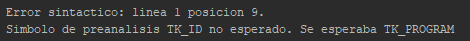
\includegraphics[scale=1]{img/sintactico/salida_sintactico_ej_error_1.png}
\caption{Salida de la ejecución del analizador sintáctico con el código de la figura \ref{fig:sintactico_ej_error_1}.}
\label{fig:sintactico_ej_error_1_salida}
\end{figure}

\begin{figure}[H]
\begin{minted}[escapeinside=||,autogobble,linenos,xleftmargin=0.35\textwidth,xrightmargin=0.35\textwidth]{pascal}
Program Example3;
Var       
    Num1, Num2, Sum : Integer;
    Result: |!Bool!|;
Begin {no semicolon}
    Sum := Num1 + Num2;
    if (Num1 > Num2) then
        Result := true
End.
\end{minted}
\caption{Programa en Pascal reducido con error sintáctico general.}
\label{fig:sintactico_ej_error_2}
\end{figure}

\begin{figure}[H]
\centering
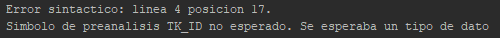
\includegraphics[scale=1]{img/sintactico/salida_sintactico_ej_error_2.png}
\caption{Salida de la ejecución del analizador sintáctico con el código de la figura \ref{fig:sintactico_ej_error_2}.}
\label{fig:sintactico_ej_error_2_salida}
\end{figure}

\begin{figure}[H]
\begin{minted}[escapeinside=||,autogobble,linenos,xleftmargin=0.35\textwidth,xrightmargin=0.35\textwidth]{pascal}
Program Example4;
|!Vars!|   
    Num1, Num2, Sum : Integer;
    Result: Boolean;
Begin {no semicolon}
    Sum := Num1 + Num2;
    if (Num1 > Num2) then
        Result := true
End.
\end{minted}
\caption{Programa en Pascal reducido con error sintáctico general y sin un token o elemento sintáctico esperado.}
\label{fig:sintactico_ej_error_3}
\end{figure}

\begin{figure}[H]
\centering
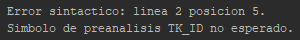
\includegraphics[scale=1]{img/sintactico/salida_sintactico_ej_error_3.png}
\caption{Salida de la ejecución del analizador sintáctico con el código de la figura \ref{fig:sintactico_ej_error_3}.}
\label{fig:sintactico_ej_error_3_salida}
\end{figure}

\section{Problemas encontrados}
Dadas las características del lenguaje, no fue posible alcanzar la clase de gramáticas LL(1), pero esto no impidió que se tomaran decisiones de diseño para poder implementar el Analizador sintáctico.

\section{Posibles mejoras}
Como mejora, en el caso de los mensajes de errores que se muestran en la compilación, debería evitarse mostrar los nombres de los tokens que se utiliza, y en su lugar deberían mostrarse los lexemas o lo que ese token representa, para ocultar aspectos de la implementación y mostrar mensajes más intuitivos.

También deberían indicarse los mensajes de error para los casos faltantes donde ``se esperaría'' un elemento sintáctico general y no un token específico.

\section{Conclusiones}
Pudimos realizar algunas modificaciones propuestas para la gramática, eliminando su recursividad a izquierda y factorizando a izquierda, pero no pudimos cumplir el requisito de que no sea ambigua, ya que el lenguaje subyacente no lo permitía. 

Más allá de no alcanzar la clase de gramáticas LL(1), el diseño y la implementación del analizador sintáctico descendente predictivo recursivo sin backtracking se pudieron concluir con éxito, tomando las decisiones pertinentes. 

Como resultado de las modificaciones sobre la gramática, ahora es más extensa y se dificulta su legibilidad y comprensión.